\section{Registrar Programa en Extenso}

Para registrar el Programa en extenso correspondiente a una Unidad de Aprendizaje, primero se da click en en la pestaña \IUbutton{Ver Tareas}. y posteriormente en el botón \IUbutton{Programa en Extenso} y la siguiente pantalla será desplegada:

\begin{figure}[!h]
    \centering
    \hypertarget{9}{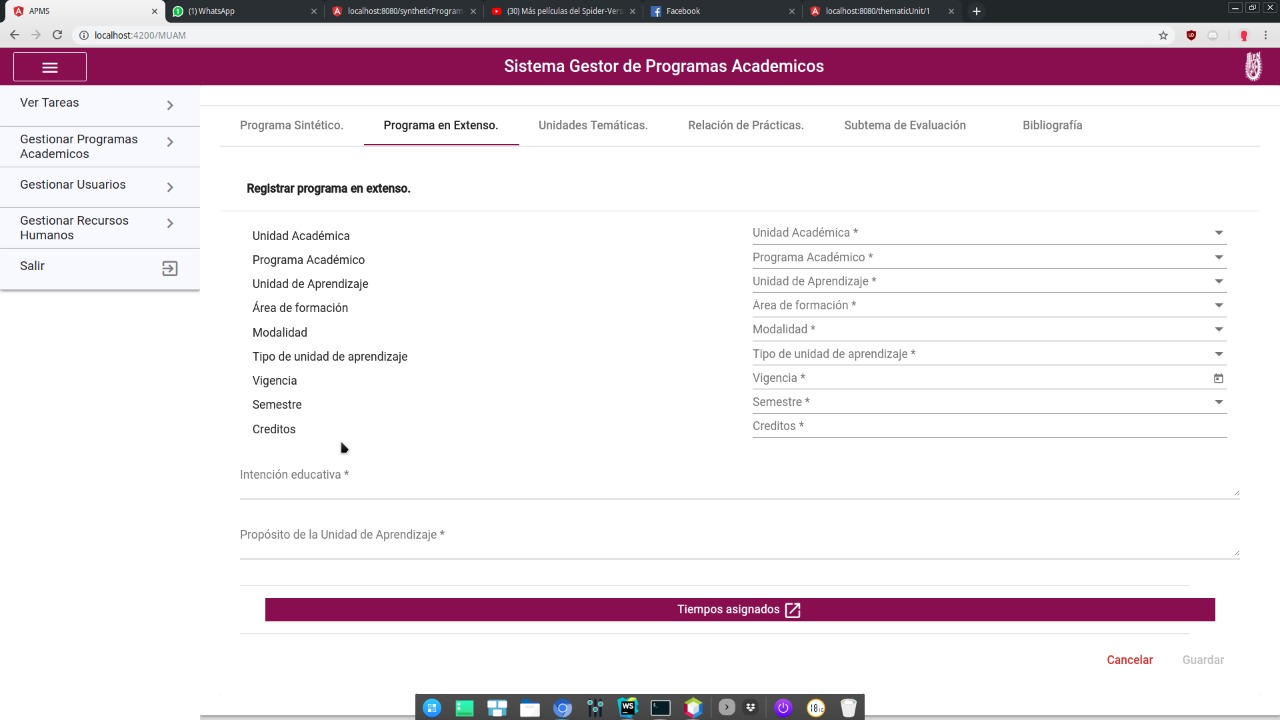
\includegraphics[width=0.5\linewidth]{images/SP6/RegistrarPS.png}}
    \caption{Pantalla Registrar Programa en Extenso}
\end{figure}

Los campos desplegados en el formulario deberan ser llenados por el Docente.

Para concluir el registro. Revisar \hyperlink{GuardarFinalizar}{Guardar y/o Finalizar}
Si hay errores checar \hyperlink{Errores}{Posibles Errores}